\documentclass{beamer}
\usetheme{CambridgeUS}

\usepackage{tikz,pgfplots}
\usepackage{amsmath,amssymb}
\usepackage{xcolor}
\usepackage{graphicx}
\usepackage{wasysym}

\title{SIKE - PQC based on isogenies}
\author{Simon Pohmann}
\institute{University of Passau}

\newcommand{\R}{\mathbb{R}}
\newcommand{\F}{\mathbb{F}}
\newcommand{\Z}{\mathbb{Z}}
\renewcommand{\O}{\mathcal{O}}

\newtheorem{prob}{Problem}

\pgfplotsset{every x tick label/.append style={font=\tiny}}
\pgfplotsset{every y tick label/.append style={font=\tiny}}

\begin{document}

\frame{\titlepage}

\section{Elliptic Curves}

\begin{frame}
\frametitle{Elliptic Curves}
Let $K$ be a field of characteristic $\neq 2, 3$.
\begin{definition}
    A (possibly nonsmooth) \emph{elliptic curve} $E$ is the zero set
    \begin{equation*}
        \{ (x, y) \ | \ F(x, y) = 0 \} \subseteq \bar{K}^2
    \end{equation*}
    of some irreducible polynomial $F(x, y) = y^2 - x^3 - Ax - B \in K[x, y]$ together with a point $\O = \infty$ at infinity.
\end{definition}
\begin{definition}
    An elliptic curve $E: y^2 = x^3 + Ax + B$ is called smooth, if the \emph{discriminant}
    \begin{equation*}
        \Delta(E) := -16(27 B^2 + 4 A^3) \neq 0
    \end{equation*}
\end{definition}
\end{frame}

\begin{frame}
\frametitle{Examples}
\begin{columns}
    \begin{column}{0.49\textwidth}
        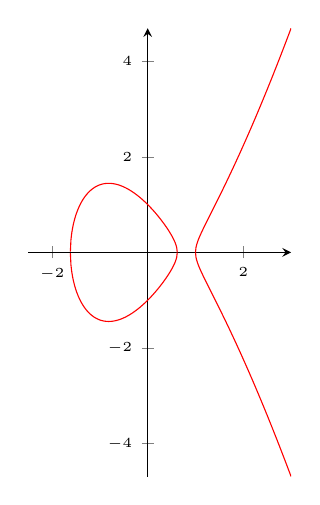
\begin{tikzpicture}
            \begin{axis}[
                axis lines = middle,
                xmin = -2.5,
                axis equal image = true,
                samples = 200
            ]
                \addplot[red, domain=1:3] {sqrt(\x*\x*\x - 2*\x + 1)};
                \addplot[red, domain=1:3] {-sqrt(\x*\x*\x - 2*\x + 1)};
                \addplot[red, domain=-1.618:0.618] {sqrt(\x*\x*\x - 2*\x + 1)};
                \addplot[red, domain=-1.618:0.618] {-sqrt(\x*\x*\x - 2*\x + 1)};
            \end{axis}
        \end{tikzpicture}

        points of $E: x^3 - 2x + 1$ in $\R^2$
    \end{column}
    \begin{column}{0.49\textwidth}
        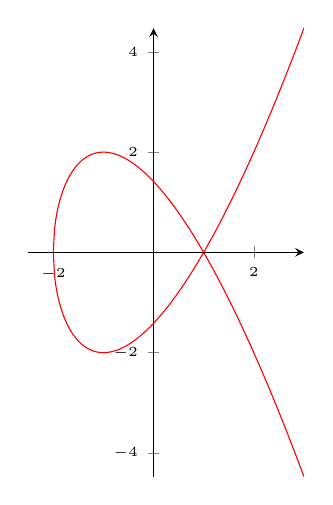
\begin{tikzpicture}
            \begin{axis}[
                axis lines = middle,
                xmin = -2.5,
                axis equal image = true,
                samples = 200
            ]
                \addplot[red, domain=-2:3] {sqrt(\x*\x*\x - 3*\x + 2)};
                \addplot[red, domain=-2:3] {-sqrt(\x*\x*\x - 3*\x + 2)};
            \end{axis}
        \end{tikzpicture}

        points of $E: x^3 - 3x + 2$ in $\R^2$
    \end{column}
\end{columns}
\end{frame}

\begin{frame}
    \frametitle{Coordinate ring}
    \begin{definition}
        Let $E: y^2 = x^3 + Ax + B$ be an elliptic curve. Then 
        \begin{equation*}
            K[E] := K[x, y] / (F), \quad F(x, y) = y^2 - x^3 - Ax - B
        \end{equation*}
        is the \emph{coordinate ring} of $E$.
    \end{definition}
    $f \in K[E]$ are the ``polynomial functions'' defined on $E$
    \begin{equation*}
        (f + gF)(x, y) = f(x, y) + \underbrace{F(x, y)}_{= 0 \ \text{if} \ (x, y) \in E} g(x, y) = f(x, y)
    \end{equation*}
    \begin{definition}
        Let $E: y^2 = x^3 + Ax + B$ be an elliptic curve. Then define the function field $K(E)$ as the quotient field of $K[E]$.
    \end{definition}
\end{frame}

\begin{frame}
    \frametitle{Rational functions - Example}
    Consider $E: y^2 = x^3 - x + 1$ and $f = \frac {(y - 1)(x + 1)} {x(x + 1)} \in K(E)$.
    
    We want to evaluate $f$.
    \begin{itemize}
        \item at $(1, 1)$
        \begin{equation*}
            f(1, 1) = \frac {(1 - 1)(1 + 1)} {1(1 + 1)} = \frac 0 2 = 0
        \end{equation*}
        \item at $(-1, -1)$
        \begin{equation*}
            f(-1, -1) = \frac {(-1 - 1)(-1 + 1)} {-1 (-1 - 1)} = \frac 0 0 \quad \text{\Huge\lightning}
        \end{equation*}
        but in $K(E)$ have
        \begin{equation*}
            \frac {(y - 1)(x + 1)} {x(x + 1)} = \frac {y - 1} {x} \ \Rightarrow \ f(-1, -1) = {-1 - 1} {-1} = 2
        \end{equation*}
    \end{itemize}
\end{frame}

\begin{frame}
    \frametitle{Rational functions - Example}
    Consider $E: y^2 = x^3 - x + 1$ and $f = \frac {(y - 1)(x + 1)} {x(x + 1)} = \frac {y - 1} {x} \in K(E)$.
    
    We want to evaluate $f$.
    \begin{itemize}
        \item at $(0, 1)$
        \begin{equation*}
            f(0, 1) = \frac {1 - 1} {0} = \frac 0 0 \quad \text{\Huge\lightning}
        \end{equation*}
        but in $K(E)$ we have $y^2 = x^3 - x + 1$ so
        \begin{equation*}
            \frac {y - 1} {x} = \frac {(y - 1)(y + 1)} {x(y + 1)} = \frac {y^2 - 1} {x(y + 1)} = \frac {x^3 - x} {x(y + 1)} = \frac {x^2 - 1} {y + 1}
        \end{equation*}
        Hence we define
        \begin{equation*}
            f(0, 1) = \frac {0 - 1} { 1 + 1} = -2
        \end{equation*}
    \end{itemize}
    
    However: $\frac 1 x \in K(E)$ cannot be defined at $(0, 1)$.
\end{frame}

\begin{frame}
    \frametitle{Morphisms}
    Now we consider maps $E \to E'$ for elliptic curves $E, E'$.
    \begin{equation*}
        \phi: E \to E', \quad (x, y) \mapsto (f(x, y), \ g(x, y)) \quad \text{for} \ f, g \in K(E)
    \end{equation*}
    These are called \emph{rational maps} or \emph{morphisms}.
    \vspace{2ex}
    \begin{itemize}
        \item $f(x, y), g(x, y)$ must fulfill the equation of $E'$ for all $(x, y) \in E$
        \\$\Rightarrow \ f, g$ fulfill the equation of $E'$ in $K(E)$ (Hilbert's Nullstellensatz)
        \item Define $\O := (\frac {\neq 0} 0, *) = (*, \frac {\neq 0} 0) = (\frac {\neq 0} 0, \frac {\neq 0} 0)$
        \\$\Rightarrow$ one can always define $f(x, y), \ g(x, y) \in E'$
        \item Write $\phi = [f, g]$
        \item What about $\phi(\O)$?
    \end{itemize}
\end{frame}

\begin{frame}
    \frametitle{Isogenies}
    Let $E, E'$ be elliptic curves.
    \begin{definition}
        A morphism $E \to E'$ that maps $\O$ to $\O$ is called \emph{isogeny}.
    \end{definition}
    \begin{definition}
        A bijective isogeny $E \to E'$ whose inverse is an isogeny is called \emph{isomorphism}.
    \end{definition}
\end{frame}

\begin{frame}
    \frametitle{Isogenies - Example}
    Let $E: y^2 = x^3 - x + 1$ and $E': y^2 = x^3 - 4x + 8$.
    \begin{equation*}
        \phi: E \to E', \quad \O \mapsto \O, \ (x, y) \mapsto (2x, \sqrt{8}y)
    \end{equation*}
    Have
    \begin{align*}
        &(\sqrt{8}y)^2 - (2x)^3 + 4(2x) - 8 = 8y^2 - 8x^3 + 8x - 8 \\
        \Rightarrow \ & (\sqrt{8}y)^2 = (2x)^3 - 4(2x) + 8 \ \text{in} \ K[E]
    \end{align*}
    So $\phi$ is a well-defined isogeny.

    Its inverse is
    \begin{equation*}
        \phi^{-1}: E' \to E, \quad \O \mapsto \O, \ (x, y) \mapsto (\frac 1 2 x, \frac 1 {\sqrt{8}} y)
    \end{equation*}
    So $\phi$ is an isomorphism.
\end{frame}

\begin{frame}
    \frametitle{j-invariant}
    Let $E: y^2 = x^3 - x + 1$ and $E': y^2 = x^3 - 4x + 8$. Then
    \begin{equation*}
        \phi: E \to E', \quad \O \mapsto \O, \ (x, y) \mapsto (2x, \sqrt{8}y)
    \end{equation*}
    is an isomorphism.
    
    Recall the discriminant
    \begin{equation*}
        \Delta(E) := -16(27 B^2 + 4 A^3) \neq 0
    \end{equation*}
    \begin{definition}
        The \emph{j-invariant} is
        \begin{equation*}
            j(E) := \frac {(-48A)^3} {\Delta(E)}
        \end{equation*}
    \end{definition}
    \begin{equation*}
        j(E) = \frac {110592} {-368} = \frac {6912} {23}, \quad j(E') = \frac {7077888} {-23552} = \frac {6912} {23}
    \end{equation*}
\end{frame}

\begin{frame}
    \frametitle{j-invariant}
    \begin{definition}
        The \emph{j-invariant} is
        \begin{equation*}
            j(E) := \frac {(-48A)^3} {\Delta(E)} = \frac {(-48A)^3} {-16(27B^2 + 4A^3)}
        \end{equation*}
    \end{definition}
    \begin{theorem}
        Two elliptic curves $E, E'$ are isomorphic if and only if $j(E) = j(E')$.
    \end{theorem}
    \textit{Proof Sketch:} Let $u^4 = \frac {A'} {A} \in \bar{K}$
    \begin{align*}
        &\Rightarrow \ A^3 (27B'^2 + 4u^{12}A^3) = u^{12} A^3 (27B^2 + 4A^3) \\
        &\Rightarrow \ u^6 = \frac {B'} {B} \\
        &\Rightarrow \ \phi: E \to E', \quad \O \mapsto \O, \ (x, y) \mapsto (u^2x, u^3y) \quad \text{is isomorphism}
    \end{align*}
    This shows $\Leftarrow$.
\end{frame}

\begin{frame}
    \begin{definition}
        The \emph{j-invariant} is
        \begin{equation*}
            j(E) := \frac {(-48A)^3} {\Delta(E)} = \frac {(-48A)^3} {-16(27B^2 + 4A^3)}
        \end{equation*}
    \end{definition}
    \begin{theorem}
        Two elliptic curves $E, E'$ are isomorphic if and only if $j(E) = j(E')$.
    \end{theorem}
    \textit{Proof Sketch:} Let $\phi: E \to E'$ isomorphism.
    \begin{align*}
        \text{Riemann-Roche Theorem} \ \Rightarrow \ \text{$\phi$ is linear}
    \end{align*}
    So $\phi = [\lambda_1 x + \lambda_2 y + \lambda 3, \ \mu_1 x + \mu_2 y + \mu_3]$
    \begin{align*}
        \text{only monomial with $y$ is $y^2$} \ &\Rightarrow \ \lambda_1 = \lambda_3 = 0 \\
        \text{no $x^2$ monomial} \ &\Rightarrow \ \mu_2 = \mu_3 = 0
    \end{align*}
    Let $u^2 = \mu_1$, then $\phi(x, y) = (u^2x, u^3y) \hfill\square$
    \\~
\end{frame}

\section{The Group Structure}

\begin{frame}
    \frametitle{Geometric Group Structure}

    \begin{columns}
        \begin{column}{0.49\textwidth}
            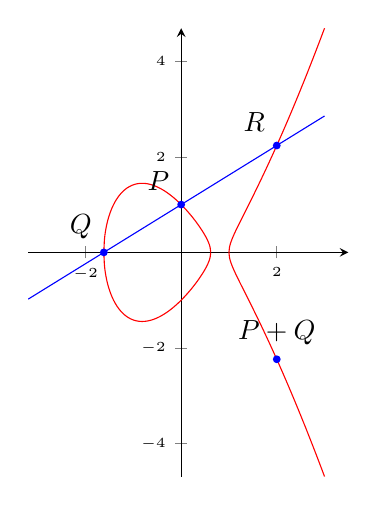
\begin{tikzpicture}
                \begin{axis}[
                    axis lines = middle,
                    axis equal image = true,
                    xmax = 3.5,
                    samples = 200
                ]
                    \addplot[red, domain=1:3] {sqrt(\x*\x*\x - 2*\x + 1)};
                    \addplot[red, domain=1:3] {-sqrt(\x*\x*\x - 2*\x + 1)};
                    \addplot[red, domain=-1.618:0.618] {sqrt(\x*\x*\x - 2*\x + 1)};
                    \addplot[red, domain=-1.618:0.618] {-sqrt(\x*\x*\x - 2*\x + 1)};

                    \node[blue, label={120:{$P$}}, circle, fill, inner sep = 1pt] at (axis cs: 0, 1) {};
                    \node[blue, label={120:{$Q$}}, circle, fill, inner sep = 1pt] at (axis cs: -1.618, 0) {};
                    \addplot[blue, domain=-3.2:3] {0.618*\x + 1};
                    \node[blue, label={120:{$R$}}, circle, fill, inner sep = 1pt] at (axis cs: 2, 2.236) {};
                    \node[blue, label={$P + Q$}, circle, fill, inner sep = 1pt] at (axis cs: 2, -2.236) {};
                \end{axis}
            \end{tikzpicture}
        \end{column}
        \begin{column}{0.49\textwidth}
            \begin{theorem}
                Each line meets $E$ in exactly three points (with multiplicity)
            \end{theorem}
            Define $P +_{\mathrm{geo}} Q$ by
            \begin{itemize}
                \item $L :=$ line through $P, Q$
                \begin{itemize}
                    \item If $P = Q$ use tangent
                \end{itemize}
                \item $R :=$ third intersection point of $L$ and $E$
                \item $P +_{\mathrm{geo}} Q := -R$
                \begin{itemize}
                    \item $-(x, y) := (x, -y)$
                \end{itemize}
            \end{itemize}
            \vspace{2ex}
            Set $\O +_{\mathrm{geo}} P = P +_{\mathrm{geo}} \O = P$.
        \end{column}
    \end{columns}
\end{frame}

\begin{frame}
    \frametitle{Algebraic Group Structure}
    From Cryptanalysis we know:
    \begin{theorem}
        The coordinate ring $K[E]$ is a Dedekind domain.
    \end{theorem}
    \begin{theorem}
        There is a bijection
        \begin{equation*}
            \rho: \mathrm{Cl}(K[E]) \to E, \quad \O \mapsto K[E], \ (\lambda, \mu) \mapsto \overline{\langle x - \lambda, y - \mu \rangle}
        \end{equation*}
        where $\mathrm{Cl}(K[E])$ is the ideal class group of $K[E]$.
    \end{theorem}
    \begin{definition}
        Define $+_{\mathrm{alg}}$ on $E$ by $P +_{\mathrm{alg}} Q = \rho^{-1}(\rho P \cdot \rho Q)$.
    \end{definition}
\end{frame}

\begin{frame}
    \frametitle{Rational Group Structure}
    Let $E: y^2 = x^3 + Ax + B$.
    
    For $P = (x_1, y_1), \ Q = (x_2, y_2) \neq -P$ define
    \begin{align*}
        \lambda &:= \begin{cases}
            \frac {y_2 - y_1} {x_2 - x_1} & \text{if} \ x_1 \neq x_2 \\
            \frac {3x_1^2 + A} {2 y_1} & \text{otherwise}
        \end{cases} \\
        x_3 &:= -x_1 - x_2 + \lambda^2 \\
        y_3 &:= -y_1 + \lambda(x_1 - x_3) \\
        P +_{\mathrm{poly}} Q &:= (x_3, y_3)
    \end{align*}
    Further $P +_{\mathrm{poly}} (-P) := \O$.
\end{frame}

\begin{frame}
    \frametitle{Elliptic Curves as Groups}

    \begin{theorem}
        Let $E$ be an elliptic curve. Then $+ := +_{\mathrm{geo}} = +_{\mathrm{alg}} = +_{\mathrm{poly}}$.
    \end{theorem}

    \begin{corollary}
        Let $E$ be an elliptic curve. Then
        \begin{itemize}
            \item $E$ with $+$ is a group
            \item $E$ is abelian
            \item $E$ has neutral element $\O$
        \end{itemize}
    \end{corollary}
    For field tower $\bar{K} | L | K$ let $E(L) := E \cap L^2 \cup \{ \O \}$ be the $L$-rational points.
    \begin{corollary}
        $E(L)$ is a subgroup of $E$
    \end{corollary}
\end{frame}

\begin{frame}
    \frametitle{Isogenies}

    Let $E, E'$ be elliptic curves.
    \begin{theorem}
        An isogeny $\phi: E \to E'$ is a group homomorphism.
    \end{theorem}

    \begin{theorem}
        Let $\Phi \leq E$ be a finite subgroup. Then there is a unique elliptic curve $\tilde{E}$ and a (separable) isogeny $\phi: E \to \tilde{E}$ with $\ker \phi = \Phi$ (up to isomorphism).
    \end{theorem}
    \begin{center}
        Write $E/\Phi = \tilde{E}$
    \end{center}

    \begin{prob}[Isogeny Path]
        Given elliptic curves $E, E'$ defined over $\F_q$ with $\#E(\F_q) = \#E'(\F_q)$, find an isogeny $E \to E'$ of smooth degree.
    \end{prob}
    \begin{center}
        smooth $\sim$ only small factors
    \end{center}
\end{frame}

\begin{frame}
    \frametitle{Idea}
    \begin{center}
        \includegraphics{scheme1.pdf}

        How to compute $E/\langle A, B \rangle$?
    \end{center}
\end{frame}

\begin{frame}
    \frametitle{Supersingular Curves}
    \begin{definition}
        Define $\mathrm{End}(E) := \{ \phi: E \to E \ | \ \phi \ \text{isogeny} \}$, equipped with addition $+$ and composition $\circ$.
    \end{definition}
    \begin{definition}
        Assume $\mathrm{char}(K) \neq 0$. Then $E$ is called supersingular, if $\mathrm{End}(K)$ is not commutative.
    \end{definition}
    \begin{theorem}
        Let $E$ be supersingular, defined over $\F_{p^2}$. If $j(E) \neq 0, 1728$ then 
        \begin{equation*}
            E\left( \F_{p^2} \right) \cong \left( \Z / (p \pm 1)\Z \right)^2
        \end{equation*}
    \end{theorem}
    We also need $E[n] := \left\{ P \in E\left(\F_{p^2}\right) \ \middle| \ \mathrm{ord}P \ | \ n \right\} \leq E\left(\F_{p^2}\right)$
\end{frame}

\begin{frame}
    \frametitle{SIDH}

    \begin{theorem}
        Let $E$ be supersingular, defined over $\F_{p^2}$. If $j(E) \neq 0, 1728$ then 
        \begin{equation*}
            E\left( \F_{p^2} \right) \cong \left( \Z / (p \pm 1)\Z \right)^2
        \end{equation*}
    \end{theorem}
    \begin{center}
        \includegraphics{scheme2_5.pdf}
    \end{center}
    \begin{equation*}
        \text{Claim:} \ E / \langle A, B \rangle \cong E / \langle B \rangle / \langle A' \rangle \ \text{where} \ A' = [m_A] \beta(P_A) + [n_A] \beta(Q_A)
    \end{equation*}
\end{frame}

\begin{frame}
    \frametitle{Correctness SIDH}
    
    \begin{center}
        \includegraphics{scheme2_5.pdf}
    \end{center}
    \begin{equation*}
        \text{Claim:} \ E / \langle A, B \rangle \cong E / \langle B \rangle / \langle A' \rangle
    \end{equation*}
    \begin{align*}
        &A' := \beta(A) = [m_A]\beta(P_A) + [n_A]\beta(Q_A), \quad \alpha': E/\langle B \rangle \to E/\langle B \rangle / \langle A' \rangle & \\
        \Rightarrow \ & \beta^{-1}(\{A'\}) = \langle B \rangle + A \quad \Rightarrow \ \ker(\alpha' \circ \beta) = \beta^{-1}(\ker \alpha') = \langle A, B \rangle & \\
        \Rightarrow \ & E / \langle A, B \rangle \cong E / \langle B \rangle / \langle A' \rangle, \ \text{hence the j-invariants are equal} &\square
    \end{align*}
\end{frame}
\end{document}